% UNIFYING THEMES: CRAFT & COLLECTIVISM

\chapter{Speculations}
\label{ch_speculations}

% This closing chapter of my dissertation will be an amalgam of works in-progress, and ideas for future work. 
\revision{Throughout my PhD studies, craft, retooling, and coproduction have been the key influences on my process. Yet my motivation has always been \textit{sustainability}}---sustainable e-textiles, sustainable manufacturing of said technology, and sustainable future communities. With the past few chapters, I've discussed how craft has been my main vehicle for engaging e-textiles design research with sustainable practices. After two subsequent chapters describing work which produced very tangible textiles artifacts, both instantiations of \textit{retooling for coproduction}, you can still ask me: how do I know that any of these results will advance sustainability in the long-term? How will Unfabricate or the Loom Pedals scale to broader e-textiles design communities?

I don't know.

I would hazard that most people today believe the universe is not deterministic, and certainly not pre-determined. We cannot know the consequences of today's actions upon the future for certain, nor see some sequence of future events already lined up. Existential musing aside, I believe that we can reasonably guess at the most probable outcomes---furthermore, we can steer present circumstances towards the more preferable futures. Activism, the very idea of driving positive societal change, would not exist without this belief. These theories of ``probable'' and ``preferable'' futures are also the foundation of \textit{speculative design} approaches, which ask designers to not only imagine the artifact they design, but also speculate on the world which houses the artifact.

\section{\revision{How Might We Coproduce Sustainable E-Textiles?}}

\revision{Speculative methods, as well as a burning desire to involve myself directly in climate action, are what fueled the rest of my work with LOOMIA's e-textiles prototyping development in 2020. The language survey discussed in Ch. \ref{ch_e-textiles} was the starting point for our collaborative study with the start-up, followed by two more phases.}

\revision{Our language survey showed that the research field itself was still forming its identity, as we did not see a consensus on whether the term "smart textiles" was in fact interchangeable with "e-textiles", or if there were other preferred terms. 
% In both AdaCAD and Unfabricate, I had chosen to use "smart textiles" in accordance with other colleagues' usage of the term as a subcategory of "e-textiles" that integrated electronics more deeply in textile structures. Thus, the opening question of this developing investigation was: who calls it "e-textiles" and who says "smart textiles"? 
The significance of language differences suggested a field that was still defining and negotiating with itself: its vision, scope, and values for the future technologies under development. As a result of this study, we formulated the term "E/ST" (e-/smart textiles) as a more expansive descriptor that would be able to hold multiple names so as to not bias discussion spaces.}
\revision{In response, we found ourselves asking: how do prototypes make their way from labs into industry and larger-scale production? What would e-textiles manufacturing look like? In 2020 (and still in 2023), the global "industry" seemed largely speculative (in both design and financial terms) without many mainstream products to serve as case studies.}

By happenstance, LOOMIA needed to run a user study of their upcoming products which were parts in a kit of e-textiles prototyping components. Coordinating with their CEO, Maddy Maxey, we found that many of our respective goals shared questions about the future of the e-textiles field, as well as the values and needs of designers, makers, and users of the technology. We combined efforts in a collaborative study that would collect qualitative data on e-textiles design practices from our associated community. In hindsight, this collaboration directly represents a coproduction between academia and industry perspectives in needs-finding and seeking out future design directions. The questions on language preferences to describe e-textiles would also provide market research for Maddy and LOOMIA; observing e-textiles designers' reactions to new prototyping components would give Laura and myself insights into how new design practices are formed; and as lab researchers and a start-up engineer, we all had lots to learn about scaling for manufacturing. 

Throughout the study, we worked in implicit and explicit inquiries into sustainability for the future of e-textiles, the result of my major concern for the field and personal investment in the cause at large. Having my central motivating agenda as this particular issue steered my efforts ultimately towards retooling and engaging with design justice discourse through speculative methods. 

\section{The Scope of E-Textiles and Sustainability}

% \section{Background}

% e-textiles and sustainability both fall across the intersections of many domains, including HCI, artistic practices, and global industry. To situate our inquiry into the intersection of these intersections, we will review key areas of research in both, as well as common perspectives in contesting open questions of what defines ``e-textiles" and what ``sustainability" means. We also briefly note how speculative tactics help practitioners interrogate these values and negotiate futures.

% \subsection{E-textiles / Smart Textiles}

% Reviews in engineering go over technological parts of how to combine them. Reviews in HCI and CSCW go into the social dimensions of what it means to combine the technologies. 
\revision{As we discussed before in Ch. \ref{ch_unfabricate}, sustainable e-textiles design faces the unique challenge of reckoning with both textile waste and e-waste. We cannot deal with such future-facing problems without first understanding their scope in the present.} Broadly defined, the e-textiles field seeks to integrate textile technologies with digital electronics. \revision{As the language survey in Ch. \ref{ch_e-textiles} explored, researchers use both ``e-textiles" and ``smart textiles", sometimes interchangeably, in the literature. This ambiguity in language blurs the already-broad scope of e-textiles, but does shed some light on where researchers' and designers' interests lie.} Potential applications include smart garments for healthcare, sportswear, and
next-generation wearable devices \cite{stoppa_wearable_2014},
as well as educational tools for teaching electronics and computational thinking through textile crafts \cite{kafai_ethnocomputing_2014, buechley_lilypad-edu_2008}. 
%  So as to not bias later discussions of this uncertainty in language, we have selected ``e-textiles" as a default.
While most of this work has occurred in lab prototypes, there have been a few examples of commercially-available e-textiles products such as Google and Levi's Project Jacquard denim jackets, and the Arduino Lilypad product line \cite{poupyrev_project_2016, buechley_lilypad_2008}. However these examples still represent specialty products, marketed towards early-adopters or those interested in making or learning how to make electronic circuits.
% LIST APPLICATIONS
While e-textiles technical development generally falls under the umbrella of pervasive or ubiquitous computing \cite{marculescu_electronic_2003}, work can be found across engineering \cite{liu_advances_2018, afroj_engineering_2019, lund_roll--roll_2018} % CITE
, textile and fashion design \cite{mcquillan_hybrid_2019, fairburn_spheres_2016} % CITE
, and human-computer interaction \cite{nachtigall_five-year_2018, posch_etextiles_2019} % CITE
and draw from multiple disciplinary vernaculars which have developed in parallel. 

Even in its present form without much of a presence in global commodity markets, sustainability is already a concern for future e-textiles. Both e-waste \cite{robinson_e-waste:_2009,forti_global_2020} and textile waste \cite{sandin_environmental_2018,muthu_textiles_2017} are established, active issues to address in combating industrially-driven environmental hazards and developing more sustainable systems. Beyond the consumption and disposal of these technologies, researchers are also concerned with wastefulness in the prototyping \cite{dew_designing_2019, wall_scrappy_2021} % CITE
and manufacturing \cite{machado_sustainable_2020, schoggl_narrative_2020}
processes that feed the industries. 
% How does the field use language, prototyping, and manufacturing as a way to collaborate on topics of interest? How can we effectively steer more conversation towards sustainability? Let's talk more about sustainability in the next section.
% Yet ``sustainability" is a broad area of research with implications for many technological fields, so we will separately review sustainability perspectives and related work, especially in HCI and creative industries.

\subsection{My Position: Sustainability means Intersectional Climate Justice}

Mainstream discussions generally conceive of contemporary human society as \textit{unsustainable}. Major industrial voices across technological sectors such as Unilever\footnote{https://www.unilever.com/planet-and-society/}, H\&M\footnote{https://hmgroup.com/sustainability/}, and STMicroelectronics\footnote{https://www.st.com/content/st\textunderscore
com/en/about/st\textunderscore
approach\textunderscore
to\textunderscore
sustainability/st\textunderscore
approach\textunderscore
to\_sustainability.html} (Europe's largest semiconductor manufacturer whose customers include Apple, Cisco, and Samsung) acknowledge the need for system-wide changes to drastically shrink their environmental impact to continue operations. % CITE from prelims
Nonprofits such as the Ellen Macarthur Foundation (whose mission is to create the ``circular economy'') and consulting firms such as Accenture (who offers ``sustainability goals'' consulting among their services) include supply chains and business values among the many infrastructural aspects that need to be transformed. In the words of system theorist Horst Rittel, attaining sustainability and averting global climate disaster is indeed a ``wicked'' problem \cite{rittel_dilemmas_1969}.

\revision{I firmly} endorse that sustainability is not only a matter of environmental regulation, but more essentially, it is justice and decolonization. As several scholar-activists have stated, the root cause of the climate crisis is capitalism -- particularly the extractive aspects of capitalism which emphasize mass exploitation of natural resources, industrialized production and distribution, and structural inequality to enforce an extremely privileged minority of humans. Rather than calling the present the ``Anthropocene", a more fitting term would be the ``Capitolocene" \cite{haraway_staying_2016, sze_environmental_2020}. Even more insightful observations come from Indigenous scholars who name that this capitalist hegemony is built upon settler-colonialism and centuries of oppression. As Kyle Whyte, a Potowatomi scholar-activist and philosopher writes, ``Anthropogenic (human-caused) climate change is an intensification of environmental change imposed on Indigenous peoples by colonialism." \cite{whyte_weaving_2016} \revision{I} subscribe to the definition that sustainability is a state of ``collaboration" between humans and environments, which expands the possible avenues for considering  humans vs. ``nature" as stakeholders in the environment \cite{kimmerer_braiding_2015, tallbear_standing_2014}.

Another reframing of an 
unsustainable system is as a failure of relationships with these other stakeholders, which then can lead to a restorative justice framework of identifying the perpetrators, auditing the harms, and working on reparations \cite{whyte_indigenous_2017}.
This framework is grounded in material consequences and tangible actions in the world, following the definition of decolonizing by Eve Tuck (Unanga\^{x}) in her influential article ``Decolonization is not a metaphor" \cite{tuck_decolonization_2012}
, that the movement to ``decolonize"  must strictly refer to returning colonized land to their original peoples and repairing Indigenous land-based relationships.
% There's lots of research on how climate change is driven by industrial processes. 
% There's also research on how climate change and environmental damage is caused by colonialism. Anti-colonialism and environmental justice are also established fields of research and activism in social justice, which have been connected back to how they are part of achieving sustainability.
% That was mostly on the sociopolitical side of how to make the world more sustainable, but 

While framing sustainability as an issue deeply entangled with other wicked social injustices may seem to frustrate the issue even further, it also connects to empowering frameworks on restorative justice, community organizing, and other tangible ways of practicing social good in everyday life, while supporting broader radical change. As activists Hi'ilei Hobart and Tamara Kneese capture in their book Radical Care, contemporary movements such as Standing Rock \#NoDAPL and Occupy have positioned themselves as ``protectors" of relationships: protecting Indigenous peoples' relationships with their ancestral lands, protecting familial relationships among undocumented migrants, and establishing their own care-based relationships to sustain these protections -- ``Care, then, is fundamental to social movements." \cite{hobart_radical_2020} Citing Angela Davis, they explain that ``individual impulses and interior lives, the intimate and banal details of family histories and personal experiences, are directly connected to external forces." By centering care and emotional investment of time and energy as a source of collective power in political organizing \cite{mcalevey_no_2016, sze_environmental_2020}, framing sustainability as an issue of intersectional justice emphasizes how people can make observable progress in their communities in addressing seemingly-intractable problems such as climate crisis.

\subsection{Current Approaches to Sustainable E-textiles}

% \todo[90\% DONE]{aligned discourses in HCI}
% there's a lot of people working on sustainability as a technological issue, too. People are studying current systems for ways that people try to work sustainably with what they have. 
Our work intersects with that of practitioners in sustainable HCI and sustainability initiatives in e-textiles industries. In designing tangible products, sustainable development must consider the material impacts of these goods throughout their lifecycles: at design (prototyping) time, during production and sourcing, in transit, and at end-of-life. Particularly for design in HCI, Lazaro et al. \cite{lazaro_sustainable_2020} describes a ``sustainable prototyping life cycle" for designers to consider the environmental impacts of different stages in prototyping and fabrication processes. One sustainable design framework which has gained traction across academia and industry is \textit{circularity}, where ``everything is a resource for something else." \cite{c2c_green_2017} As a fundamental reconfiguration of the notion of ``lifecycle", circular design has generated supporting concepts such as ``remanufacturing" \cite{nasr_fundamentals_2020} and ``reverse supply chains" \cite{battaia_reverse_2015}. Sustainable HCI provides several tools that reckon with such an epistemological shift towards \textit{sustainable interaction design} \cite{blevis_sustainable_2007}, such as a framework for understanding sustainable social practices \cite{entwistle_beyond_2015}, ``disintermediation" as a design rubric for interaction design \cite{raghavan_means_2017}, and alternative evaluation methods for ``usability" that considers alternative product lifecycles \cite{remy_evaluation_2018}. These tools promote sustainable values and mindsets for designers of digital technologies, as well as users of these sociotechnical systems. 

Specific to textiles and fashion, designers are generally aware of the unsustainability of the global industry and engaging with the aforementioned sustainable design strategies \cite{brydges_closing_2021, kohler_challenges_2013, veske_review_2020}. e-textiles practitioners have explored the unique affordances of textiles for sustainable design tactics, such as the ability to repair textiles-based technologies by darning \cite{jones_e-darning_2021} and inherent structural compatibility with \textit{designing for disassembly} \cite{wu_unfabricate_2020}. Designers in e-textiles (and more broadly in textiles/fashion) recognize the particular social dimensions in which their artifacts are situated, so research on sustainable textiles often emphasizes personal relationships, intimate bodily contact, and sentimental value -- for example, Fletcher's \textit{Craft of Use} \cite{fletcher_craft_2016} and Kuusk's work on service-based, personalized production of sustainable smart textiles \cite{kuusk_crafting_2015}. Expanding beyond individual practices, sustainable textiles has found homes in collaborative, distributed efforts including the EU Wear Sustain Network \cite{goodman_wear_2018} between artists and industry, and textile waste marketplaces like Queen of Raw \footnote{https://www.queenofraw.com/} and Fab Scrap \footnote{https://fabscrap.org}.

% They're also trying to design more sustainable systems to replace the present ones. One example of a design approach is circularity. People talk about the ``circular economy" and what systems, infrastructures, and policies need to be changed or rebuilt to make it happen. 

% Other design approaches are ``modularity", ``recycling", ``reusability", ``biodegradability", and other features of sustainable design. We see these as tactics that might be future components of sustainability.

% These sustainable tools and concepts are propagated 

% --add a few sentences here marking how we intersect with sustainable HCI, sustainability and speculation, and sustainable e-textiles initiatives. 
% something about how HCI has been tackling sustainability and efforts currently in place to support sustainable textiles (EU wear sustain, Queen of Raw, Fab Scrap)}

Given the intersectional nature of sustainability, and the entangled histories of textiles and computing development with global inequities as previously discussed, we also find relevant discourses in the HCI for Development (HCI4D) and Postcolonial Computing communities. In examining the distinct methodological challenges from the Global North \cite{chetty_hci4d_2007}, research in the Global South vitally explores issues of alternative infrastructures for craft \cite{jack_infrastructure_2017, zhang_designing_2019}, and the disproportionate impact of industrial waste \cite{rifat_breaking_2019} and colonial legacies \cite{philip_postcolonial_2012, irani_postcolonial_2010}, directly related to sustainable e-textiles's responsibility to reckon with the global inequity driving industrialized climate change.

% Through these research projects, I have created techniques, software, and hardware tools to upgrade and maintain the vehicle. Yet, a souped-up vehicle does 

% Sustainability can be a nebulous, distant goal, and I lean into this uncertainty by designing for sustainability through \keyterm{speculative} methods. 

% brain dump:
% key motivating ideal in my research is sustainability, but specifically I believe that sustainability = intersectional climate justice
% in solidarity with Indigenous activists, restorative justice practices, and many intersectional approaches which center how ``sustainability" does not only speak to environmental impact, but collective wellbeing of humans along with the more-than-human. 

% intro section for chapter is a political rant pretty much
% cite environmental justice sources, Indigenous/Black + POC-led activism, design justice

% how it has appeared through my research?

% starting with methods: a lot of concern (anxiety) about equity for human participants in my studies, leading to a lot of "freeform" interactions that fell outside of the structured standard procedures of interviews, participant compensation, paper authorship...

% - started in LOOMIA study
% - Loom Pedals study

% Consistently reviews rated me "low" in rigor, struggling to communicate the subversive intent in research practices in typical academic terms


% paste in LOOMIA interview stuff here

% why speculative methods
% summarize e-textiles language



% 2.3.1 	Coproducing Smart Textiles Through Conversations

% Our study was divided into three segments, each targeting a component of e-textiles practice to investigate for existing sustainability dialogue and thinking, along with potential development. These segments were (1) Language used by practitioners to describe the e-textiles domain, (2) practices in Prototyping future e-textiles technologies, and (3) perspectives on future e-textiles Manufacturing at scale. Each segment of the study centered around conversations between e-textiles practitioners (ourselves included), aiming to uncover and solicit reflections on the values in their design practices.

% The first Language segment was conducted via an anonymous online survey sent to both LOOMIA's and the lab's combined networks to seek out as many perspectives as possible. Participants were asked for non-identifying demographic information such as age, nationality, educational background, current job title, and years in the e-textiles field – all of which gave context to how "experienced" they saw themselves in the practice, given that expertise in a young, interdisciplinary field could be so subjective. They were then asked about which terms – out of "smart textiles", "e-textiles", "flexible hybrid electronics", "functional fabrics", and others – that they were aware of, used in their practice, and if they had any preferences or distinctions between them. Furthermore, the survey participants were asked for other language-based associations of e-textiles technology, such as the most desirable features (e.g. softness, washability) and most commonly-advertised application domains. 
% After receiving over 60 in-depth survey responses where most participants had filled completely-optional free-response text questions, we felt it was appropriate to close the Language segment by inviting the participants to non-anonymously attend a virtual "E-Textiles Town Hall" event where they could meet not only us, the researchers, but also others in the e-textiles community. The event was structured as an interactive webinar where Maddy and I presented the participants with a summary and initial analysis of their responses, including demographic context. The face-to-face real-time interaction with an actively-engaged audience confirmed a suspicion I held while reading the survey responses: that while e-textiles was an exciting domain for innovation and career advancement, hence the wide variety of disciplines that carried in and adapted their jargon; many practitioners also held a personal stake in the field outside of technical and economic interests and may deeply value certain directions for the technology, such as assistive wearables for the care of elderly relatives. Thus, the language differences within e-textiles also reflected the differing emotional and social dynamics of practitioners.

% Next, the Prototyping segment was conducted as a "Beta Test" of LOOMIA's component prototypes which were about to be put into production and released to the public. Nine participants were recruited from people who had been actively engaged with the company's communications on these components (e.g. responding to customer surveys, reacting on social media), and who were interested in trying out the products in exchange for their feedback on their design and supporting documentation. I personally worked with each participant virtually, meeting them in Zoom calls for interviews and collaborating remotely in Google cloud documents, over the course of several weeks during the summer of 2020. While I could meet everyone, know the identities of participants and acquaint myself with their personal stories, participants were kept anonymous to Maddy to preserve the confidentiality of their feedback and to minimize LOOMIA's liability as a non-research organization. As such, any materials refer to them with pseudonyms.
% Simultaneously with the Prototyping interviews, the Manufacturing segment consisted of a series of unstructured interviews with e-textiles "manufacturing experts", defined as anyone working in e-textiles who had interacted with manufacturing entities to attempt (and in most cases, fail) to bring an e-textiles product to market. Similarly to the Prototyping segment, we also use pseudonyms for the participants. We recruited from the Unstable Design lab's professional networks (mostly Laura's), leveraging Laura's position as tenure-track faculty and thus, relatively senior and well-connected in e-textiles, to identify other practitioners who had some combination of research and product development experience. Fig 18 displays the one-on-one participant interactions, which I led for both interview segments, as "business cards", recalling how the unstructured nature of these interviews felt like a casual, but professional, coffee conversation between newly-acquainted colleagues.

% In these conversations, I was more explicitly able to target values that individual e-textiles practitioners held in their own design practices. Yet as a result of framing these research interactions as interpersonal ones, they were also subject to dynamics such as "polite" conversation and "feeling out" the conversation partner's position before broaching potentially-polarizing (and in mainstream discussions, "politics" that are not currently integrated into "tech") topics such as racial diversity and sustainability. Overall, our study did not show that sustainability had a significant presence within the values of e-textiles practice. Rather, the central finding throughout all three segments of our study was how forming and maintaining personal relationships was a common strategy for e-textiles practitioners to meet challenges such as disciplinary boundaries, access to specialized spaces, and gaps in expertise. Each of the three aspects of e-textiles practice we observed -- language, prototyping, and manufacturing -- represented different influences on the nature of these collaborative relationships. 
% How interpersonal relationships drive human goals is a topic of study in many fields, from scientific and technological development [89,119,131,150] to political movements [58,91,134]. Yet in retrospect, I also see how spotlighting the role of relationships in this emergent technology also speaks to how the e-textiles discipline is a coproduction: that one does not make e-textiles without also asking "what is an e-textile?", defining one's own sense of the field and one's own professional associations in the process.

% 2.3.2 	Speculative Retooling
Despite the lack of overt values related to sustainability, we see this key finding about relationships as a promising means to connect our conversations among e-textiles practitioners to threads of sustainability in other discourses. In order to show the breadth of these connections as a potential foundation for sustainable e-textiles development, we discuss the specific findings in the context of a speculative vision of a sustainable e-textiles discipline. 
% Our methods borrowed elements of qualitative interviews  and thematic analysis [20,21] in social research to collect participant data. We use the term speculative construction to describe our primary tactic for bridging these qualitative methods with speculative methods to envision a sustainable e-textiles community of practice. Foremost, our vision centers design justice [33] and finds roots in observations about current practices and politics of e-textiles. The "speculative" component draws from speculative design, notably summarized in Dunne \& Raby's Speculative Everything [43] and often overlapping with design fiction, which has been taken up in HCI to push design beyond specific objects to consider designed artifacts as ideas that suggest possible futures and systems, as well as alternative presents and histories [2,12,142]. A core value in speculative design is considering the wide array of possible futures and identifying the plausible futures for deeper speculation. Out of these plausible ones, researchers can inquire into preferable futures aligned with certain values. We use user interviews and observations to guide our viewfinder to "plausible" futures, and design justice to focus on "preferable" futures.

% In this process, we trace the usual speculative futures path backwards to the originating point of Dunne \& Raby's and Candy's "possibility cone" or "futures cone", located in the present. However, applying a lens of intersectional justice shows us that there is not simply one singular way to experience the present due to multiple axes of systemic oppression, placing individuals at different coordinates along race, gender, class, etc. To complicate the present, and foreground social justice, of which sustainability is a critical part, we looked to Costanza-Chock's Design Justice, which describes a matrix of domination that selects for more socially privileged design perspectives, separating design sites into the privileged (e.g. Silicon Valley, university hackathons) and the subaltern (e.g. auto shops, weaving studios). We believe that design justice magnifies the present point so that it no longer appears to be a singularity. Instead, it is now a debris field of alternate histories and possibilities truncated by past violence, illustrated in Fig. 19. This connection led us to look beyond success stories to uncover more humble points of pride, as well as frustration, and failure. 

% Prior research has also taken up speculative methods to center sustainable values. Especially relevant to our study of sustainability in emergent technology is Liu et al.'s exploration of "collaborative survival" [85], stemming from a speculative design inquiry in pushing sociotechnical entanglements towards more ``preferable" sustainable futures, as well as Wong et al.'s toolset for ``infrastructural speculations" [148]. Both of these works offered us tactics for inquiring into a context for an emergent technology such as e-textiles that considers the complex, often-fraught sociopolitical factors that make sustainability such a wicked problem. 

\section{Where Does Sustainability Fit?}

The survey results and analysis ultimately suggested the \textit{latent} themes within e-textiles practices \cite{corbin_grounded_1990} --- values which designers might not explicitly voice, but are implicitly embedded into the work. Our findings are inconclusive on whether those in the e-textiles field are actively thinking about sustainability. However, we get a strong sense that the technology will be highly personal: designers also see themselves as future users, and that interactions should be materially pleasurable. 

Even compared to 2020, sustainability has become a much more mainstream topic in public discourse. Thus, I would be curious how participants would respond today.
Since conducting this survey, my own opinions on the language of e-textiles have shifted a couple of times. At the time of my dissertation proposal, I chose to use ``smart textiles'' for consistency with my publications. However, more recently, my preferences have shifted towards ``e-textiles'', disillusioned with the ``smart'' descriptor.

\section{Methods: Crafting a Speculative Construction}

\begin{figure}
  \centering
  
\includegraphics[height=2.5in]{figs/EST_Future Cone.png}
  \caption[Illustration combining the ``futures cone'' from speculative design with design justice's acknowledgement of historical violence.]{An expanded view of the beginning of the futures cone \cite{dunne_speculative_2013}, showing that the "present" arises from messy histories of truncated possibilities, once futures to a past point in time.}
  \label{fig:justice-futures-cone}
\end{figure}

Our methods incorporated elements of qualitative interviews \cite{braun_online_2020, fontana_interviewing_2007} and thematic analysis \cite{maguire_doing_2017, braun_using_2006} in social research to collect participant data.
We use the term \keyterm{speculative construction} to describe our primary generative tactic for bridging these qualitative observations with ideas from design justice and speculative design to envision a sustainable e-textiles community of practice. Foremost, our vision centers \citedterm{design justice} \cite{costanza-chock_design_2020} and finds roots in observed practices and politics of e-textiles. The ``speculative" component alludes to \citedterm{speculative design}, notably summarized in Dunne \& Raby's \textit{Speculative Everything} \cite{dunne_speculative_2013} and often overlapping with \textit{design fiction}, which has been taken up in HCI to push design beyond specific objects to consider designed artifacts as ideas that suggest possible futures and systems, as well as alternative presents and histories \cite{akama_speculative_2016, baumann_infrastructures_2017, wakkary_sustainable_2013}. However, we specifically describe this work as \textit{speculative} rather than a full \textit{speculation}, as we do not present a coherent design world but still draw on the methodology's core concepts.

One such core value in speculative design is considering the wide array of \textit{possible} futures and identifying the \textit{plausible} futures for deeper speculation. Out of these plausible ones, researchers can inquire into \textit{preferable} futures aligned with certain values. We use our data to guide our viewfinder to "plausible" futures, and design justice to focus on "preferable" futures.
Prior research has also taken up speculative methods to center sustainable values. Especially relevant to our study of sustainability in emergent technology is Liu et al.'s exploration of ``collaborative survival" \cite{liu_design_2018}, stemming from a speculative design inquiry in pushing sociotechnical entanglements towards more ``preferable" sustainable futures, as well as Wong et al.'s toolset for ``infrastructural speculations" \cite{wong_infrastructural_2020}. Both of these works offered us tactics for inquiring into a context for an emergent technology such as e-textiles that considers the complex, often-fraught sociopolitical factors that make sustainability such a wicked problem. 

Where design justice enriches speculative design's framework is at the originating point of %and Stuart Candy 
the ``possibility cone" or ``futures cone" from Dunne \& Raby and Stuart Candy\cite{dunne_speculative_2013}, located in the present. Applying a lens of intersectional justice shows us that there is not simply one singular way to experience the present due to multiple axes of systemic oppression, placing individuals at different coordinates along race, gender, class, etc. To complicate the present, and foreground social justice (of which sustainability is a critical part), Costanza-Chock's elaboration of \textit{design justice} \cite{costanza-chock_design_2020} describes a \citedterm{matrix of domination} that selects for more socially privileged design perspectives, separating design sites into the \textit{privileged} (e.g. Silicon Valley, university hackathons) and the \textit{subaltern} (e.g. auto shops, weaving studios). We believe that design justice magnifies the present point so that it no longer appears to be a singularity. Instead, it is now a debris field of alternate histories and possibilities truncated by past violence.
% , illustrated in Fig. \ref{fig:justice-futures-cone}. 
Broadening the speculative cone allows us to look beyond success stories to uncover more humble points of pride, as well as frustration, and failure -- thus expanding our sense of possible futures. Furthermore, design justice's core strategy of \textit{retooling} -- designing tools that dismantle the established matrix of domination and construct a new, justice-oriented sociotechnical order -- offers a framework for designing these tools as components for building further speculation, hence the ``construction" descriptor for our analysis.



% can you say something here about what the difference between speculation and design recommendations? 


% sw - what I learned from making this graphic is that sometimes, making a graphic can help me write a section, even if the graphic doesn't make it into the final paper

% combine with submerged perspectives (Decolonial Perspectives) and subaltern design sites (Design Justice) -- adding in justice as a metric for "preferability" of a future


\section{Interviewing E-Textiles Makers}

To briefly review the first leg of the study, the language survey described in Ch. \ref{ch_e-textiles}, our collaboration is broadly concerned with the future of e-textiles, particularly its growth as a technology and its sustainability. Our research question focused on how sustainability could manifest materially and implicitly for e-textiles designers. 
% As e-textiles practitioners ourselves studying practices in our own network, this study was designed for the authors' two interrelated purposes: to inform product development for a growing e-textiles market, and to survey implicit design values within the discipline, such as manufacturability and sustainability. Both goals concern the future of e-textiles as it ``scales" as a technology and social practice. While the study's data collection did not specifically target sustainability as a design value, the research question that emerged to guide our analysis and reflections can be summarized as follows.


% In this section, we will describe these methods in a chronological narrative of our research process. To preserve confidentiality (especially in ensuring honest product feedback), all participant data was anonymized by the principal investigator, A1, and given pseudonyms for dissemination.
% \begin{figure}[h]
%     \centering
%     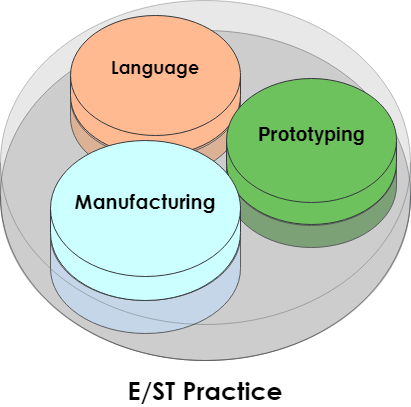
\includegraphics[width=2.5in]{figs/EST_Study Design.png}
%     \caption{A study design targeting three distinct components of e-textiles practice: language, prototyping, and manufacturing. The graphic shows the components as completely separate entities merely for clarity. The components represent distinct, but possibly overlapping and entangled aspects which e-textiles practitioners encounter.}
%     \label{fig:study-design}
% \end{figure}
The study's three segments each targeted a component of e-textiles practice to investigate for existing sustainability dialogue and thinking, along with potential development. These segments were (1) \textbf{language} used by practitioners to describe the e-textiles domain, (2) practices in \textbf{prototyping} future e-textiles technologies, and (3) perspectives on future e-textiles \textbf{manufacturing} at scale. These latter two segments relied on personal interviews between myself and the participants, resulting in rich, but extremely unstructured data.
% However, as our research questions sought possibilities rather than generalizable

\subsection{Prototyping}
% After concluding the language segment, we moved onto the prototyping segment. This sequencing was purely pragmatic, as the user test involved Flexsu sending sample products to the participants and the company needed the lead time to produce enough inventory. To study e-textiles prototyping, we leveraged Flexsu's "beta test" framing of the pre-release user test of their product line. 

In studying prototyping practices, we aimed to assess the values (which may or may not include sustainability) that e-textiles practitioners brought into their prototypes and ideas of future technologies.
We drew upon established user testing methods in human-centered design for products \cite{shneiderman_designing_2016, buley_user_2013} such as usability metrics and application-specific heuristics. %However, we combined these conventions with tactics from speculative design \cite{dunne_speculative_2013} and critical technical practice \cite{agre_toward_1997}, which deconstruct notions of ``usability" and ``product value" in order to probe beyond designing for a consumer product, into a design's sociotechnical context and its relationships with human agents. 
We used these methods to jointly evaluate LOOMIA's product line, which included pressure sensors, digital press buttons, heating elements, and various connectors, all based on a flexible substrate that could conform to a soft textile surface, and probe the participants' ideas for possible applications. Each beta tester received two different components from the company, which would allow them to evaluate LOOMIA's technology in two differing form factors and/or functions. 
% With two components, the participants would also be able to evaluate the connection techniques designed for the components. 
Data on the beta testers' experiences and from their direct feedback were collected in one round of introductory interviews, a 3-week period of remote, asynchronous observation by the authors, and a second round of exit interviews.  During the interviews, we used tactics from reflective design \cite{sengers_reflective_2005} and cultural probes \cite{boehner_how_2007} to prompt participants to deconstruct notions of ``usability" and ``product value" in order to probe beyond designing for a consumer product, into a design's sociotechnical context and its relationships with human agents. 

%\begin{figure}[ht]
%    \centering
%    
\includegraphics[width=3in]{figures/400x150.jpg}
%    \caption{Flexsu's product line of prototyping components. [image omitted for review]}
%    \label{fig:prototyping-components}
%\end{figure}

During the remote observation period, I gathered additional data through interacting with the participants in Slack and video calls in which they helped participants troubleshoot the components, gathering image/video documentation of their prototyping process.
All of the participant data was transcribed (or captured/downloaded for messages and multimedia), anonymized to preserve the confidentiality of the participants, then shared amongst all of the authors to review. We performed a thematic analysis of this qualitative data, identifying shared and differing aspects of participants' experiences within each study group, as well as comparing themes across the study segments. In the parlance of Braun \& Clarke's method for thematic analysis, we paid especially close attention to the ``latent" themes (what the participants \textit{meant} in the data or \textit{why} they said it) that underlaid the ``semantic" themes in the data (\textit{what} the participants said) \cite{braun_using_2006, maguire_doing_2017}. To address the RQ, we investigated whether or not ``sustainability" was among the latent themes observed.

% \subsubsection{Recruitment and Introductory Interviews}

% Prior to our collaboration, Flexsu had sent preliminary interest surveys to their subscribers to gauge potential customer interest in certain types of components (e.g. pressure sensors, connector buses, heaters), and to solicit potential participants in a user test. Based on these communications, A2 had identified a list of contacts who were consistently responsive and openly provided feedback. A1 recruited the beta testers from this list, keeping the final list of nine participants and their feedback anonymous to A2.

% Once each participant had received their components from Flexsu, A1 scheduled the first interview with them in a Zoom video call. The unstructured format of the introductory interviews allowed the meeting to progress much like an initial meeting between new colleagues. A1's questions about the participants' individual work and what interests brought them into their current position. Moving into the present context of the study, participants were asked how they found out about Flexsu, and what ideas they had for the components that they would be testing. Overall, these questions sought to generate a sense of the participants' interdisciplinary trajectories, grounded in their personal stories. The hope was also to use this first conversation to establish that A1 was interested in maintaining contact throughout the beta test period, as well as a collaborative relationship as fellow e-textiles practitioners continuing beyond the study, if they so desired.

% \subsubsection{Follow-up: Participant Observation, Exit Interviews, and Beyond}

% The introductory interviews also served as orientations for the participant observation stage, gauging each participant's interest and capacity for additional interactions with A1 or the other participants. To scaffold the participants' experimentation with the Flexsu components, the authors provided written design prompts and technical documentation. Additionally, when recruiting for the beta test, A1 had offered personalized ``help time" for the beta testers as an informal incentive, where they would be available to meet virtually for electronics tutorials or project consultations. After more than half of the participants indicated interest in some form of group communication to meet each other and suggested the platform, A1 also created a Slack workspace for the beta testers. 
% Then I sat back and hoped that they would actually use the components over a couple of weeks. 
% The prompts were written from my experience with conventional UX design thinking, trying to slip in some more critical design and cultural probes. 
% Didn't get a whole lot of engagement in Slack, but a couple of interesting questions, documentation of their experimentation process, and one participant used the "help time".
% Everone was super busy so there were only four exit interviews (one from someone who missed their intro). There were two people who were product design focused, one who was definitely academic, one who was in product design but was more focused on her personal learning
% At end of the three week remote observation period, A1 reached back out to the participants to schedule an optional exit interview which would include more formal product evaluation questions. 
% Interestingly, one participant who couldn't make an exit interview did so because he was going to a big protest, which went along with his intro interview mentioning how he had trouble making sure his political activism was compatible with working as a maker.
% After the beta test was formally over, I kept in touch with most of the participants because again, they were cool.

\subsection{Manufacturing}

Finally, in the Manufacturing segment we sought a deeper understanding of the existing landscape for e-textiles manufacturing, as a combination of electronics and textiles manufacturing sectors. How is sustainability considered in this landscape, and what are the barriers that impede sustainable e-textiles development (or scaling e-textiles technologies in general)? We recruited ``manufacturing experts" for this segment, keeping our criteria for an ``expert" intentionally flexible due to the lack of e-textiles products that have gone to mainstream markets. Participants were recruited based on our familiarity with their work in e-textiles and manufacturing, as well as the diversity of opinions and perspectives they might bring to our speculations for future e-textiles sustainability.
% The final segment of our study was initiated during the Participant Observation stage of the Prototyping segment, as we used the lull in facilitating direct interactions with participants to recruit participants for a set of interviews about e-textiles manufacturing. 

We conducted this segment using unstructured interviews to keep the conversational space open to each interviewees' unique experiences. A1 conducted these interviews as one-on-one video calls where the primary goal was to engage the interviewee in a casual, but in-depth conversation where they felt comfortable in reflecting on their personal motivations in their work. This approach borrows from unstructured qualitative interviewing in cultural anthropology, which are often used in conjunction with ethnographic fieldwork to develop an empathetic understanding between the researcher and participant \cite{fontana_interviewing_2007, gburgess_unstructured_1982}. More recent anthropological work from practitioners with marginalized experiences expands upon these methods to challenge disciplinary power inequities, such as Kim TallBear's feminist, Indigenous approaches to inquiry of ``standing with" and ``speaking as faith" \cite{tallbear_standing_2014} to attend to differences in privilege and analyze power dynamics between researcher and participant. 
The goal of the manufacturing interviews was not to generate into a representative model of the manufacturing ``landscape" in a structured, systematic fashion. Rather, this dialogic, associative procedure was used to generate a set of unique perspectives with a few interviews and limited time. Together with critical activist scholarship in social research, this conversational method was well-suited for drawing out systemic factors in the participants' stories.

% don't discuss submerged perspectives and design justice yet, just considering those as part of futuring/alternate past-presents

\section{Findings: the Centrality of Relationships}

We summarize our findings through the lens of the study's central finding and recurring theme:
% Overall, our study is inconclusive on whether sustainability has a significant presence within the values of e-textiles practice, but does suggest which values may be currently emphasized. 
how forming and maintaining personal relationships was a common strategy for participants to meet challenges such as disciplinary boundaries, access to specialized spaces, and gaps in expertise. While we are unable to draw a conclusion on whether sustainability has a significant role within e-textiles design values, this key finding about relationships has fueled our reflections on similar themes found in other discourses, many of which are overtly focused on sustainability. 

Each of the three aspects of e-textiles practice we observed -- language, prototyping, and manufacturing -- represented different influences on the nature of these collaborative relationships. How interpersonal relationships drive human goals is a topic of study in many fields, from scientific and technological development \cite{rifat_breaking_2019, steinhardt_breaking_2016, maudet_design_2017, zhang_designing_2019} 
to political movements \cite{hobart_radical_2020, sze_environmental_2020, mcalevey_no_2016}, comprising an important vehicle by which humans construct and arrange societal values. 
We see this value of relationships, observed in our conversations among e-textiles practitioners, as a promising foundation for a community of practice that actively engages with issues of sustainability, material impact, and other social issues as part of e-textiles design. In the following section, we will discuss the specific findings from each segment to situate the speculative construction in our discussion. 

%These connections are made as \textit{speculations}, grounded in our \textit{observations} from interacting with study participants, forming what we will call a \textbf{\textit{speculative construction}} of our local e-textiles community of practice. Leaning into the various meanings of `construction' in HCI, we will employ a metaphor of designing and building a house to present how interpersonal relationships factored into each component of the e-textiles ``house".

% \begin{figure}[h]
%     \centering
%     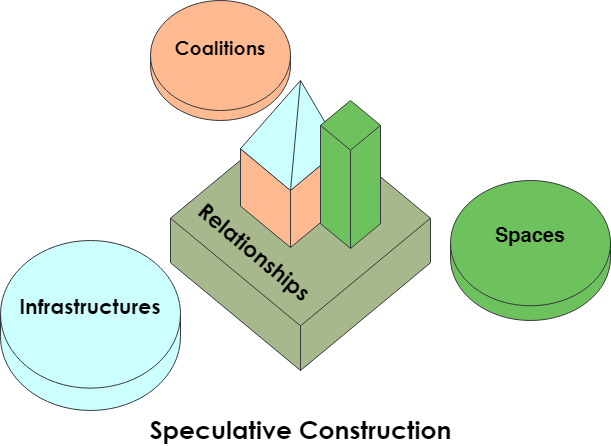
\includegraphics[width=3in]{figs/EST_Findings.png}
%     \caption{Conceptual illustration of a \textit{speculative construction} for an e-textiles practice built explicitly upon valuing relationships between practitioners. The three components of practice from Fig. \ref{fig:study-design} have been used to suggest three configurations of social relationships: coalitions, spaces, and infrastructures.}
%     \label{fig:findings-specConstruction}
% \end{figure}



\subsection{Prototyping: Materials First, Sustainability (and Other Values) Later}
The data from the Prototyping segment consisted of audio recordings of all interviews: 8 introductory interviews and 4 exit interviews, totalling 12 hours of interviews with nine participants. Roughly separating the beta testers by their primary interest in participating, we studied a mix of people interested in learning basic electronics for hands-on professional development (n=2), design research inquiry (n=2), exploring technical challenges (n=2), and designing consumer products (n=3).
Beginning from the introductory interviews of the prototyping segment, we saw a recurring theme of movement into and within e-textiles in the participants' career trajectories. 
%It was though, if e-textiles was a house, they headed towards upon entry, what helped make them comfortable, or what made the space intimidating.
Beyond learning how to work with a new material or even a new application or tool, many participants were challenged with a whole new domain of knowledge. For example, Sydney and Gary were experienced product designers for a particular domain (textiles and workplace ergonomics, respectively), but neither had ever designed electronic devices. This element of getting acquainted with a new field was reflected across other introductory interviews. Participants shared what about the e-textiles field had piqued their interest in coming over from another field, such as those who dealt with product design -- who saw e-textiles as an upcoming trend that would be applied to the markets they worked in: home furnishings (Dorian), acoustics (Xander), educational tools (Eli), and wearable devices (Jack).

In summary, these interviews presented e-textiles as a space of possibility for career development and creative experimentation. Yet, as participants described their design ideas, from heated therapy cushions to gesture-sensing fabrics, sustainability did not seem to factor into their thought process. The participants were amenable to thinking about sustainability when A1 mentioned their own design values, and would share their thoughts freely. However, their responses to sustainability (as well as broader issues of equity) as factors in their design process suggested that it, along with cost, scalability, and aesthetic theme, were considerations for the ``next version" (Dorian) of the prototype. The exit interviews, which revealed that many of the participants had not even gotten to physically work with the components because they needed to obtain a soldering iron or first decide on a project concept, suggested that the foremost values in the early stages of prototyping are product viability and technical feasibility. 

We imagine that sustainability and other values can be relegated to secondary or incidental factors when material considerations, such as soldering a connection or measuring pressure sensitivity, are immediately tangible and visible to the designer. Even Odette, who teaches e-textiles concepts and researches critical values in fashion technology design, connected sustainable e-textiles to ``triple bottom-line economics" and other theoretical, abstract concepts, rather than her immediate prototyping concept. The focus on prototyping and learning may have allowed participants to "bracket off" concerns for broader distribution, where sustainability might be more foregrounded. Additionally, the products with which they engaged did not have specific aesthetics or branding focusing on sustainable design (such as the use of natural materials or "green" branding). We see a possible space to question where sustainability could be a more explicit value in a design process. For one, the aesthetics of a prototyping tool might suggest different possible applications for such tools. Also, returning to our theme of relationships in shaping e-textiles practice, the participants' personal relationships generated their first project ideas (e.g. designing for a pet or to aid a loved one's health struggle) and guided them to enter e-textiles in the first place. Hector and Sydney, both senior professionals in their fields, cited wanting to ``keep up" with A2's work as reason for exploring e-textiles applications.

% \begin{figure}[h]
%     \centering
%     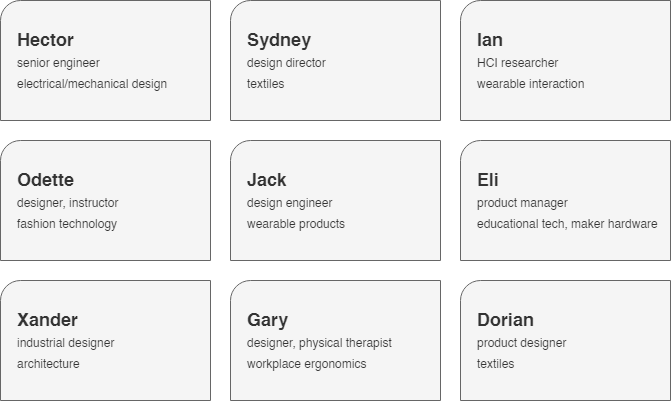
\includegraphics[width=3in]{figs/EST_Beta Test.png}
%     \caption{Roster of all nine beta test participants, formatted as ``business cards" that associate each participant with their pseudonym, job description, and development focus.}
%     \label{fig:beta-test-roster}
% \end{figure}


% The two interested primarily in professional development were Sydney and Eli. Sydney is a professional textile designer working at a multinational textiles manufacturing and distribution company. Over her career, she has advanced from designing products to directing product innovation in her current position. Sydney has been in touch with A2 and Flexsu for some time, following the growing potential of e-textiles entering her work in textiles manufacturing.
% Eli is an educational technology % ed-tech?
% developer who taught himself programming while working in consumer electronics retail, then moved into development at start-ups in maker-oriented and educational products (e.g. 3D printers). 

% Both design researchers were also the only two beta testers working in academia: Ian and Odette. Ian is a researcher in HCI interested in wearable and textile computing applications for artistic, expressive, and embodied interactions, who took a particular interest in the pressure-sensing matrices. 

% The first beta tester that I met with was Hector, a veteran engineer with experience in mechanical engineering, electrical engineering, consulting, and even art over the past two decades. Having followed new areas of innovations for so long, his recent work had taken a turn towards textile and wearable applications. 

% Lastly, comprising the product design set was Gary, Xander, and Dorian, who were product designers in different domains: workplace ergonomics, industrial and architectural design, and home textiles, respectively. Dorian was the only beta tester not in the USA, located in Germany. 

% Of note is the fact that all of the beta testers, except for Jack, were older than A1.
% we saw the beta testers bring different values for their process, like product design, personal learning, and design research.
% In the beta testing process, we were able to directly observe the participants learn how to design with a novel component. However, beyond learning how to work with a new material or even a new application or tool, many participants were challenged with a whole new domain of knowledge. For example, Sydney and Gary were experienced product designers for a particular domain (textiles and workplace ergonomics, respectively), but neither had ever designed electronic devices. This element of getting acquainted with a new field was reflected across other introductory interviews. Participants shared what about the e-textiles field had piqued their interest in coming over from another field. % TODO find quotes
% Most of the professional product designers -- Sydney, Gary, Eli, Xander, Dorian, and Jack -- saw e-textiles as an upcoming trend that would be applied to the markets they worked in, such as home furnishings (Dorian), acoustics (Xander), educational tools (Eli), and wearable devices (Jack).
% Jack and Hector -- more engineering-focused, while Jack was closer to the application side, but both saw e-textiles as a source of technical challenges which was more interesting to them than end-use applications
% A1 brought in my own values too, which is how sustainability and equity was a part of the space, but it didn't really seem like other people were bringing those in as their goals
% prototyping felt like a very free space for exploration and experimentation, maybe a little too intimidating for some people.
% what are some of those scary things? how can tools and kits make them better?

% TODO: connect sustainability, not explicit or really present in "latent" themes, but personal relationships is a potential "in" with sensitive or new topics


\subsection{Manufacturing: Gatekeeping and Templated Relationships}
Lastly, the Manufacturing segment's data consisted of 7 interview recordings and transcripts (one of which was with Maddy). 
% As Mars said, the manufacturing interviews were like interviews about how people didn't like manufacturing. It's like a template that products have to try to fit themselves in
Our sense of the landscape of e-textiles manufacturing is one where designers, production workers, and even factory management are disempowered in forming their desired relationships to further their goals for sustainability. It was as if manufacturing paradigms imposed a "template" that one has to fit in order to successfully manufacture in e-textiles, leaving little room to consider sustainability in that process. Kent, a designer and academic researcher in fashion technology, had worked in both high-street fashion and research labs and was familiar with supply chains in both textiles and consumer electronics. The template has been strict and merciless with his designs: through trial and error, with emphasis on \textit{error}, he had "one thing out of twenty years make it to market" during his career in fashion. For Bridget, a textile designer who had started at a large sportswear company in research and development (R\&D), sustainability was about conforming to regulations. Bridget described how her workplace's sustainability measures were largely facilitated by a ``directory" of expert personnel who specifically handled regulatory compliance and legal matters. As a production sewist, Mars felt that manufacturing removed the social value embodied in small scale hand work. They observed how garments were designed to be ``operationalized" into discrete stages, reducing possible inconsistencies between workers but also removing the ``weird nitty gritty details" of experimentation which they so enjoyed about craft work. Normative values and established practices often got in the way of the participants' ideas of sustainability and social good.  However, press was one factor that helped ease these burdens. Maddy described how LOOMIA had gotten "a lot of press", which caught the attention of their current manufacturer, who initiated the collaboration. Without this interest, they would have had to convince the manufacturer to "have some sort of faith" in the potential product. 

Another start-up leader also suggested that success or failure for their start-ups was strongly determined by external agents such as manufacturing and supply chain executives, who served as gatekeepers. Rikki, an early-career engineer who was developing a textile recycling start-up, saw opportunities for reducing the environmental impacts of textiles manufacturing, while introducing changes that could enable larger-scale restructuring in the industry. Despite the environmental and financial benefits, and the technical feasibility of her work, the most challenging aspect of industrial-scale production for Rikki was engineering a network of human contacts that would support the start-up. In actively navigating existing manufacturing ecosystems, both A2's and Rikki's organizations struggled with achieving a production volume that would sway potential manufacturers. Furthermore, most small companies cannot afford specialized personnel to handle the details (e.g. quantifiable emissions, non-use of certain materials) for desirable certifications. However, A2 pointed out that factories need to consider their ``tooling costs" when adapting for new product, leading them to impose gatekeeping criteria (e.g. quantity) in order to meet their own needs. We observed that gatekeeping could arise as a response to one's own external constraints, creating the need to know the "right people" and leading entrepreneurs to wonder, "How do I convince the [purchaser for the manufacturer/lead designer/some innovation lead] to invest in my idea?" Generally, the more powerful ``big players" with the regulatory or social capital to promote sustainable development have little incentive to initiate progressive relationships, entrenched as they are by legal and financial privilege.

However, the instances of sustainable enterprises that succeed or at least persist, e.g. Lenzing as cited by Rikki and heritage artisans as cited by Kent, suggest that working outside of the manufacturing template is not totally impossible.
With his knowledge of different product supply chains, Kent identified aspects of present-day manufacturing processes which are already shifting. He pointed to the trade-offs which the semiconductor industry has made in order to achieve its scale in volume and uniformity: materials are sourced from every inhabited continent and shipped to hyper-specialized nodes in the supply chain (a handful of foundries across the globe produce integrated chips). The rise of alternate manufacturing models such as Industry 4.0 and community-based tabletop manufacturing \cite{machado_sustainable_2020, kohtala_making_2017} is already challenging this paradigm and redistributing infrastructure. For Anais, the director of a fashion tech start-up in Europe that combines design, prototyping, and small-scale manufacturing, the response was to bring different parts of the design cycle under one roof. For Anais, change needed to actively consider scale--she expressed that "a prototype isn't enough" for making social impact, especially for a wicked problem such as sustainable development, and one needed to create a middle space where the "scaling" between prototype and product was itself an area of inquiry. Others looked to other, complementary modes of engagement, as a means of making impact. For instance, Freia, a university professor, shared that her work in hardware development had fundamentally been about "getting out into the real world". Her current community-based work also effected social change through technology and design, but felt more "exciting" and critically engaged than "manufacturing and distributing hardware". In pushing against the limits of the manufacturing template and finding it to be "not enough" for achieving the systemic change they desired, the manufacturing interviewees were already offering their own speculations for alternative systems. 
% She noted that, working directly with communities whose traditional artisan craft practices have persisted despite the proliferation of mechanized, industrialized commodity production, modern textiles have an especially long history of privileging very select practices and marginalizing the rest.
% The most commonly cited cause of failure for a manufacturing project was the failure to establish relationships with the correct people. As we will discuss in the findings, the structures that obstructed these relationships also obstruct the participants' efforts in sustainable development.
% \begin{figure}[h]
%     \centering
%     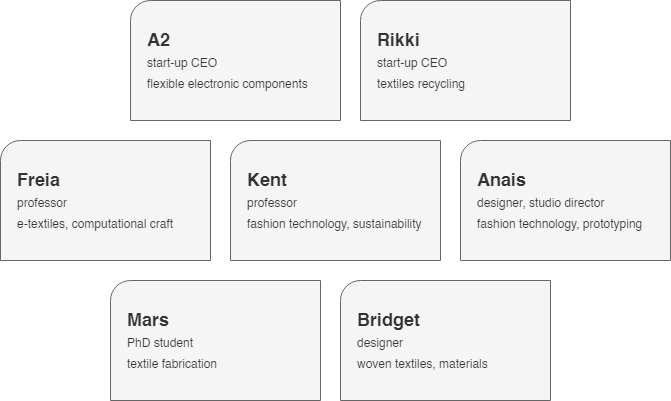
\includegraphics[width=3in]{figs/EST_Manufacturing.png}
%     \caption{Business card roster of all seven manufacturing interviewees. [A2 anonymized for submission]}
%     \label{fig:manufacturing-roster}
% \end{figure}
% SUMMARY
We observed this ``manufacturing" template, as an existing barrier for electronics and textiles development, is an even greater barrier to \textit{sustainable} e-textiles development. Our ``relationships" theme not only manifests as a common tactic for navigating the present landscape of manufacturing, but also as a concept for philosophical speculation: how can we practice relationships differently to re-envision ``manufacturing" for sustainability? 
% In total, the study collected roughly 22 hours of participant engagement through interviews or other real-time interactions over five weeks during the summer of 2020.

\begin{figure}[h!]
  \centering
  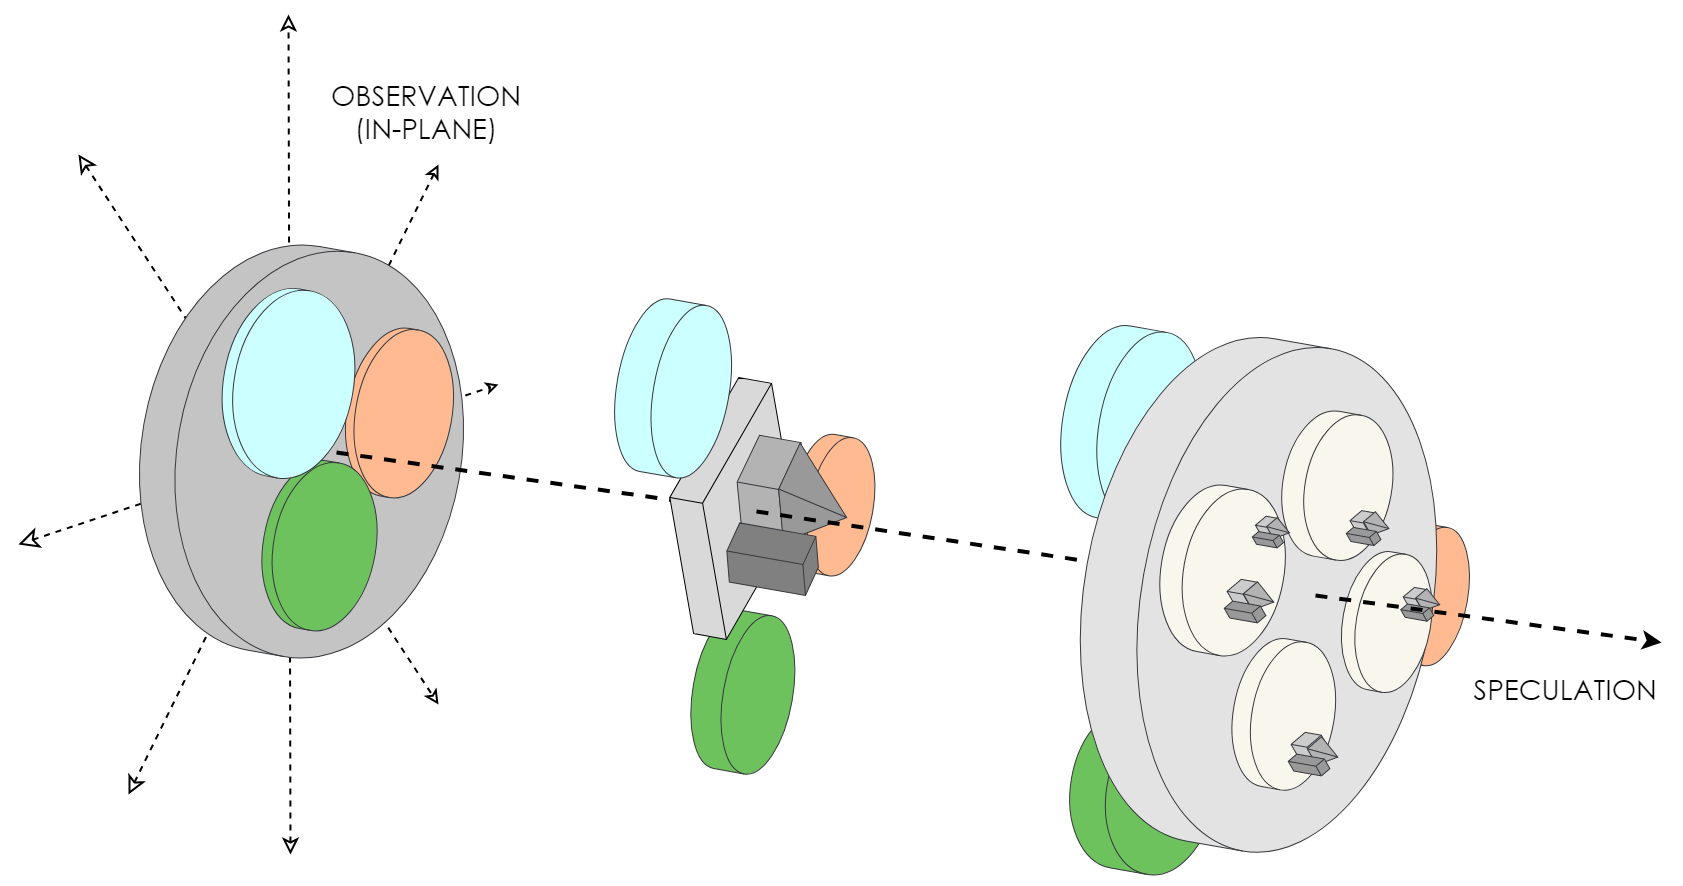
\includegraphics[width=\textwidth]{figs/EST_Discussion.png}
  \caption[Conceptual map of the progression of ideas in the E-Textiles \& Speculations study.]{%\todo[labels in pic?]{} 
  A conceptual map of the progression of ideas in the study described in Chapters \ref{ch_e-textiles} and \ref{ch_speculations}. We identified three aspects of e-textiles practice (left) to study. Our observations of such (middle) revealed a central theme of relationships. Reflecting on our findings, we used ``relationships" as a core value of a \textit{speculative construction} (right) of sustainable e-textiles design, envisioning how current aspects of practice may be retooled to foreground sustainability through relationship-building.}
  \label{fig:spec-visioning}
\end{figure}

\section{Discussion: Retooling for Sustainable e-textiles}
While we did not observe that sustainability has an overt presence in e-textiles language, prototyping, and manufacturing practices, our participants certainly valued relationships as part of e-textiles practice: as a means of bringing and transmitting values such as sustainability, and also as a philosophical component of a sustainability mindset. From these observations of potential e-textiles compatibility with sustainable development, we present our discussion as a %we employ our tactic of 
\keyterm{speculative construction} for doing sustainability within e-textiles's community of practice, drawing out implicit disciplinary values into explicit material engagement. 

We believe that framing the discussion as a speculative set of concepts, rather than a list of questions, immediate design lessons, or even a fully-developed speculation, helps us refer back to Costanza-Chock's main recommendation for design justice: \textit{retooling}. As examples of a retooling agenda for justice-oriented AI, Costanza-Chock names developing ``intersectional user stories, testing approaches, training data, ... among many other tools" \cite{costanza-chock_design_2020} that counter and dismantle the normative tools provided by the matrix of domination. A speculative construction helps us develop a similar agenda for sustainable e-textiles by identifying specific components of a possible practice. In Fig. \ref{fig:spec-visioning}, we illustrate how we see these speculative components arise from the existing components in the Findings section. We recognize the tension between the imaginary, sometimes absurd nature of speculation and the concrete action that social justice demands. To reckon with this tension, we took inspiration from similarly speculative aspects of visions for justice-oriented preferable futures, orienting our speculations towards possible outcomes of collective action movements that we might begin in the present. We particularly looked to Ghoshal et al.'s work on information \& communication technology (ICT) practices in grassroots organizing spaces \cite{ghoshal_toward_2020}, which suggests a possible synthesis of ICT development and grassroots social justice practices. Following these voices, we propose a general ethos for sustainable e-textiles design practices, which we will develop further in this section: \textbf{"Build relationships first, then tools."} 
Our speculation, then, envisions retooled aspects of e-textiles development that leverage related threads in HCI. 




In the following speculative scenes, our vision of \keyterm{retooling for sustainable e-textiles} implements the theme of ``relationships" as \textit{interconnections} -- whether between humans, non-human lives, devices, or systems -- and explicitly integrate sustainability to form tools in a future ecosystem for sustainable e-textiles. These tools address an observed need in our e-textiles community of practice, while also advancing a broader cause in a global context. Our story begins with the ``us" assembled through the study: the authors, the E-Textiles Town Hall participants, the beta testers, and the manufacturing experts. We ask, ``What if?" What if we keep these conversations going? What if we formed a sustainable e-textiles coalition to demand manufacturing change? Thus, the first design tool arising from considering relationships in the practice is not software or hardware, but rather a social configuration. From this beginning, we describe scenes set around a sustainable e-textiles ``workbench" being outfitted with this speculative toolset, suggesting the social and technical formations that emerge. We will regularly look to political organizing and social justice activism to speculate on how these visions can inform actions in the present, empowering people to orient themselves towards a longer-term ideal that is beyond the more urgent, and often bleak-seeming, present.  

  % say something of how that factors in here - maybe that speculation allows us to orient towards a longer term, perhaps idealistic goal, rather than focusing on the more immediate, and somewhat hopeless, present. 
% To organize our observations into suitable grounds for speculation, we looked to two concepts which have significant bodies of literature. (1) Our observations took place within our \textit{community of practice} of e-textiles, situating our study in our own networks and positionalities \cite{wenger_communities_1999, barton_beyond_2005}. (2) We assumed a constructivist stance aligned with the \textit{social construction of technology} -- that materials, technological, and social realities are all inextricably linked and shape one another, rather than one deterministically causing another (e.g. technology dictating social practices). A constructivist stance lends itself to asking ``normative questions" about existing power structures and the political status quo \cite{bijker_social_2012} in order to distinguish the non-normative alternatives. 
% \begin{figure}[ht]
%     \centering
%     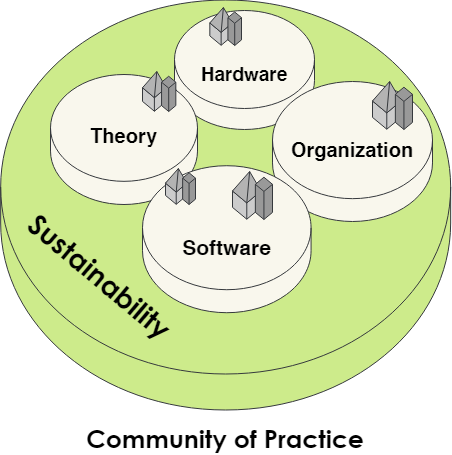
\includegraphics[width=2.5in]{figs/EST_Opportunities.png}
%     \caption{A speculative relationship-based toolset for doing sustainable e-textiles development for a community of practice.}
%     \label{fig:opportunities}
% \end{figure}
% As designers, we want to go back to making things, so here's some opportunities for further study and development, AND to discuss sustainability explicitly in the field

\subsection{Tool 1: We Form a Coalition for Sustainable E-Textiles}
As in community organizing, we start with ourselves and the people around us, where we are most able to build a base of power.
% } -- a factory worker from China, a PhD student from North America, an e-waste recycler from Ghana, a European textile artist, an Indigenous Brazilian hardware hacker, and many others\footnotemark --
 In order to stock the workbench with sustainability tools that also dismantle the unequal privileges between us, we form a \textit{coalition} -- 
% \footnotetext{These individuals are hypothetical, but based on studies of e-textiles, ICT, and HCI practices \cite{ lindtner_reconstituting_2016, carlson_ewaste-worker_2016, renno_activism_nodate, fairburn_spheres_2016} in different regions and disciplines.}
an association formed between groups with different identities, but shared goals. 
These groups may share a bigger umbrella identity (often emerging from the coalition itself), but the group identities are distinct under aggregation. 

Our Manufacturing participants shared with us a sense of disempowerment as the "small" players in a field of enormous corporate entities that upheld the unsustainable manufacturing status quo, and they are hardly alone. Coalitions for sustainability are emerging globally as a strategy for building enough collective power in grassroots movements to effect institutional and legislative change \cite{noauthor_movement_nodate, hess_sustainability_2014}. We looked to examples of successful (and failed) political coalition efforts in modern history to see that forming and sustaining these social configurations is hard, to put it lightly. Effective coalitions such as the Third World Liberation Front organized Black, Chicano, and Asian university students to  strike in 1968, laying the foundations for ethnic studies as an academic discipline \cite{npr_student_nodate}. However, coalitions that fall short, such as the 1955 Bandung Conference between 29 African and Asian nations to organize against colonialism, can end up creating a false sense of solidarity that only feeds the injustices they seek to change \cite{nopper_illusion_2015}. Coalitions are organized relationships; according to this scholarship, a successful coalition is a reciprocal relationship between the concerned groups, a value widely held in social justice discourses including HCI \cite{dombrowski_social_2016} and Indigenous-led climate justice \cite{hobart_radical_2020, whyte_indigenous_2017, gomez-barris_extractive_2017}.

Uniting under a common group identity and negotiating differences in values is a key feature of political movement-building. Rarely does a single group achieve political change without building alliances with other organizations \cite{post_multi-organizational_2015} and acting as part of a collective. The Language segment of our study showed differences in lived experiences that reflect similar dynamics in these historical coalitions. 
Inspired by the contested space of e-textiles language, we envision that, rather adopting a definitive group identity, e-textiles can leverage this ``dissensus" (from adversarial design \cite{disalvo_adversarial_2015}) to acknowledge the multitude of disciplinary perspectives in the space and maintain a productive level of critical engagement with sustainability. As Robin Wall Kimmerer writes in \textit{Braiding Sweetgrass} on the ``grammar of animacy" (speaking about relationships between humans, land, and more-than-human beings as living connections \cite{kimmerer_braiding_2015}), everyday language can be seen as a tactic for embedding reciprocal, sustainable values into cultural practices. As an interdisciplinary, emergent field, e-textiles is already positioned to become a coalition of disciplines working towards shared development goals. %\todo[relate back to our findings (esp. Language)] The disagreement in terms shows that coalition is difficult but suggests an opporutnity to suggest terms that  
By leaning into language disagreements as opportunities to find terms that highlight values (as opposed to application domains),
% the existing practices of relationship-building to collaborate within the field, 
practitioners can foreground sustainability and incorporate principles of reciprocity and equity learned from social justice movements to align the community ethos with sustainable development.

\subsection{Tool 2: We Establish Community Spaces for Growth}

By starting with a workbench for sustainable e-textiles, we realize that the stakeholders need a location to house it. Beyond a physical site, they also need to construct a social space with norms that facilitate reciprocal, equitable relationships while working at the table.
% housing cooperatives, networks and norms
% AORTA alliance for anti-oppressive trainings
Particularly in the Prototyping segment, we saw a need for a virtual communal space to discuss e-textiles practice, allowing for diverse knowledge frameworks to accommodate for different backgrounds. In this scene, such spaces have developed out of existing communities such as the E-Textiles Summer Camps \cite{noauthor_httpetextile-summercamporg_nodate} and activist hackerspaces \cite{renno_activism_nodate}, connected virtually by equally experimental networks evolved from eReuse.org \cite{franquesa_circular_2016}, where members can exchange and document sustainable tools, materials, and practices with practitioners in different spaces.
These spaces allow people to enter sustainable e-textiles with a variety of disciplinary perspectives, holding a place for them whether they come from design or production, electrical engineering or textiles or waste management. 
% Lots of research out there on building better educational spaces, including ones for professional development.

As discussions of diversity, equity, and inclusion (DEI -- sometimes ``JEDI" to include justice, too) become more mainstream in professional, as well as personal and educational, contexts, we have many potential resources to draw upon. Digital organizations such as All Tech is Human, which seeks to build the "responsible tech pipeline" \footnote{https://alltechishuman.org/} and the Intersectional Environmentalist \footnote{https://www.intersectionalenvironmentalist.com/}, promote values of DEI, sustainability, and other ethical concerns in multidisciplinary virtual forums and webinars. Similarly, community activism spaces, such as cooperative housing networks that engage with housing justice, compile resources for shared responsibilities, healthy communication, and conflict mediation \cite{nahc_national_nodate, aorta_aorta_2021} to maintain inclusive, pluralistic spaces.
The value of such spaces for promoting education, critical reflection, and prosocial behaviors has been extensively studied in educational and organization research, including settings outside of traditional classrooms such as situated ``communities of practice" \cite{wenger_communities_1999}.
We also see seeds of compatible thinking in existing interaction design and industry methods for sustainability. These spaces may borrow from "Agile" workflows which democratically "letting the actors involved find out what works or not" rather than top-down managers \cite{rolland_scaling_2016}. As another example, a handbook of sustainability in textiles technologies draws connections between ``lean" manufacturing mindsets and low-waste sustainability \cite{muthu_textiles_2017}. Lean methods have been taken up by various communities of practice, including start-up communities which A2 is a part of \cite{ries_lean_2011} which emphasize building a ``community" through direct product feedback and integrating design/development and user engagement in the same space. With careful cultivation, even parts of present-day manufacturing practice may be fruitful for sustainable development. We survey this array of spaces which all host discursive seeds for sustainability to suggest that, in addition to pursuing tooling agendas, HCI might also find a deeper understanding of sociotechnical innovation in activist spaces that lie outside of privileged design sites.


% As discussed in the speculations from our Prototyping observations, an immediately actionable opportunity is to create and experiment with community spaces for e-textiles. In fact, work in this regard has been underway for years through the E-Textiles Summer Camp (link) % TODO: CITE or note
% , classroom spaces, and other scattered groups around the globe. We recognize the potential for a future multi-sited ethnography of e-textiles practices in these spaces, perhaps inquiring into global perspectives and cultural influences on how sustainability is conceptualized in relation to the material practices of e-textiles.
% Flexsu's doing a Discord server and workshops

% There's also lots of writing out there in how-to books for UX designers and prototyping people, "agile" or "lean" processes. <find sources, or as A2 for any faves> 
% AND there's stuff that holistically talks about learning spaces intersecting with identities like race and gender, how to address power differences due to marginalization (DEI). So if we want to talk about sustainability in this intersectional sense, this literature could help.


%ld - no new data here ;) In our own practices, we are exploring different collaborative structures for building community within our own networks. Of note, A2, after an initial limited-run release of Flexsu's products, created a Discord server as a backchannel for prototyping workshops that they would offer as a service with their components. Members of the server show some initial interest in developing more of a discussion forum outside of the workshops, so we are interested in seeing how this space develops, and how future inquiries might support the formation of a community.

% Looking to sources which we have already referenced in this paper, and other related work, we propose the following starting points as sites of experimentation:

% \textbf{How can e-textiles spaces create educational resources that engage sustainability in a social and collaborative manner?} Especially with the field's emergent nature, not only are new materials surfacing frequently, but novel (to the space) ideas and techniques which may be carried in from other domains. These resources might build upon invaluable reference materials, such as those on KOBAKANT, with discussion and support spaces that facilitate supportive relationships around learning to navigate complex issues.

% \textbf{How might sustainable e-textiles spaces practice design justice and question conventions of documentation and codification?} As discussed in accounting for design justice in a speculative framework, a sociotechnical field will contain marginalized spaces and subaltern design sites resulting from existing inequities. Taking cues from radical spaces 

\subsection{Tool 3: We Build Hardware Components to Ease Hard-Soft Connections}
% my flexible hard-soft connections spiel
Finally, after building the workbench and a home for a network of relationships to grow for a sustainable e-textiles community of practice, we can finally build what are more conventionally considered ``tools". One such project is directly inspired by a conversation I had with one of the beta testers. The Prototyping segment highlights a hardware challenge present both in our speculative universe, as well as present e-textiles development: the physical act of connecting digital electronic hardware (often made of rigid polymers and metals) to textile objects (e.g. fabrics, cushions, yarns which are usually soft and flexible). This material barrier has been discussed at length by practitioners in e-textiles, even warranting a category of techniques under the label "hard-soft connections" \cite{kobakant_hardsoft_nodate}.
If we consider that mixing materials and bonding hard-soft interfaces with adhesives makes disassembly, recycling, and sustainably manufacturing more difficult \cite{soh_design_2014, battaia_reverse_2015}
, then hard-soft connections are not only the critical component of e-textiles functionalities, but could also be a critical deciding factor in the sustainability of future e-textiles products.

In the Prototyping segment, we observed how electrical hard-soft connections were a major source of cognitive friction for the beta testers, preventing many from even starting their physical prototype. Additionally, several Manufacturing interviewees expressed frustration that hard-soft connections were often too bulky, or too fragile, or just too messy, which prevents prototypes and products that are comfortable, durable, and aesthetically pleasing.
Inspired by the concept of ``interposers" from a beta tester, Hector, in contextualizing his work, we envision our future as one in which flexible microprocessor interposers can adapt existing rigid processors (e.g. Arduino boards) to a textile surface. Interposers, and the related ``carrier boards" and ``breakout boards" were existing tactics in embedded systems engineering that have been effective in facilitating physical interconnects and modular systems, from pre-2000 semiconductor manufacturing \cite{semiconductor_khandros_1992} to recent advances in flexible electronics \cite{souriau_wafer_2019, vervust_integration_2012}. Interposers in existing smart garments represent a system-wide hard-soft connection between the digital electronics and the textiles, reducing the technical development needed to make an e-textiles device washable through modularity. 

Translating the interposer model to prototyping and development tools in e-textiles would extend flexibility, durability, and overall textile compatibility to any component that could potentially be used in an application. One iteration of the carrier board system might use LOOMIA's printed substrate technology to create bases that are designed for different board footprints. We can build on the work of present-day e-textiles hardware such as the Lilypad and Adafruit platforms \cite{buechley_lilypad_2008, posch_etextiles_2019, jones_wearable_2020}, which leverage textile techniques to create "sewable" circuits, in searching for textile-friendly components for the physical connectors. The carrier would use strong, yet releasable mechanical connectors to hold the processor module, while allowing it (the most sensitive component of an e-textiles system) to be removed and replaced. 
% Here, we are returning to a thread from the beta testers' struggles with choosing and using microprocessors for an e-textiles prototype. After showing participants the KOBAKANT page on hard-soft connections that appropriate a variety of metal components across textiles (findings, zippers, snaps, etc.) for electronics use, we wondered why there were not more "hacks" for adapting and appropriating electronic components for textile use. 
Developing this carrier board is then ideologically facilitating hard-soft connections between the material worlds of electronics and textiles, creating a more fluid disciplinary interface.


% While thus far in issuing this challenge, we have not mentioned sustainability, notice that we have mentioned "modularity" and "washability" as features carried over from an interposer model. Modularity, reusability, and maintain-ability are all design tactics for sustainable systems, reducing resource consumption throughout an item's lifecycle <sources> % CITE
% . By focusing development into creating hard-soft connections that are more durable and can be repeatedly connected/disconnected, we can enable more reliable modular designs and reusable prototypes in e-textiles. Lastly, to reiterate our reflections, all of these interconnections are to facilitate more connections between people to build power in a movement for sustainable e-textiles development. Hardware development could provide a hands-on avenue for technical disciplines to engage with sustainability by interrogating the environmental impacts of their materials, their place in global supply chains, and who is (not) in their networks of practice.

% \subsection{Scene 4: We Design Software Tools that Foreground Material Impact}

% Besides hardware tools, we also develop software with our sustainable e-textiles colleagues.
% Another design need which we observed, particularly in the Prototyping segment, is that creating conceptual or software interconnects between system components was also difficult. We need better ways to visualize connections and networks in these assemblages of hardware and software, cloud and local data, and soft and rigid design paradigms.

% % As one possible avenue for addressing this issue, we propose creating software (or perhaps mixed-reality) tools to visualize on-body or in-environment circuits. Taking Flexsu's products as an example, one could envision a make-your-own-pack applet for bus connectors on a vendor's website, where users might sketch paths on application-specific templates. An potential reference would be the online schematic maker by Digi-key, one of the top three largest online electronic components vendors in North America (note link) % TODO: add footnote
% % . The tool primarily serves to assist shoppers in ordering the correct parts from Digi-key's extensive inventory, and while we make no claims about the design implications beyond these preliminary observations, it provokes questions in interface design on how to link finite materials to theoretically infinite design simulations.

% An inspirational example for these software tools that could connect different systems is Fritzing\footnote{https://fritzing.org/} \cite{knorig_fritzing_2009}% 
% , a circuit design program shown to be accessible to many skill levels because of its visual representations of multiple views (e.g. schematic, PCB) when integrating components. Furthermore, HCI research in computer-assisted design (CAD) has shown how multiple views in software tools can not only assist designers in troubleshooting \cite{strasnick_coupling_2021}, but also engage them in material or broader-scope considerations such as reusing waste \cite{wall_scrappy_2021}, designing textile structures, \cite{friske_adacad:_2019}, and scaling for manufacturing \cite{khurana_beyond_2020}.
% % Another notable feature is community contributions, where new circuit parts can be democratically added in by users, resulting in models of many switches, sensors, and even textile components.

% We imagine complementary views that allow a designer to toggle between functional digital design and material constraints, such as switching between a view of a circuit's schematic and a view of the project's bills of material (BOM), can help designers take stock of material implements from different disciplines and domains. In assembling systems out of components that come from complex, historied infrastructures in textiles and electronics, such as sourcing waterproof fabrics alongside high-frequency sensors, such tools can expose users to the material and environmental impacts of their designs and develop tacit experience with sustainable design.

% \subsection{Scene 5: We Practice Mutual Aid in ``Manufacturing"}

% In this final scene, we listen in on the conversations around the workbench to find that they are quite plausible to conduct, even in the present. Here, we intentionally blur a speculative ideal and a recommended tactic in practicing \textit{mutual aid} when producing our e-textiles artifacts. As an inspirational riff, we offer a principle from this form of community-based resource sharing: practicing mutual aid with one's neighbors is ``[helping] each other build the world we both will live in" \cite{leander_bindewald_httpswwwmutualaidnetworkorg_nodate}.

% While the Manufacturing segment revealed several challenges to future sustainable e-textiles production, we also observed how these challenges developed the participants' critical awareness of the systemic factors that drove their struggles. We envision methods by which ``manufacturing" provokes thought and subsequent engagement in making change at the system- and infrastructural-level. Ghoshal et al.'s work points out how a grassroots orientation towards ``inclusivity" generates ``beliefs, practices, and artifacts" which generate an emergent technoculture \cite{ghoshal_toward_2020}. We offer one such synthesis by explicitly discussing reciprocity and equity in each transaction we carry out when prototyping or manufacturing e-textiles technology. In doing so, we practice this sustainable vision in embodied, locally impactful ways.


\section{Limitations: Our Positionality}

The scenes at our sustainable e-textiles workbench represent an appropriately incomplete selection of possible tools. While we attempt to incorporate diverse viewpoints in our speculative construction, our methods and analysis through relationships is limited by our own subjective positions.
% In the research process, several considerations were made for the authors' circumstances. First, our mixed team of academic and industry positions  encountered friction between these structures right at the outset of our collaboration, while proposing this study to an Institutional Review Board (IRB). The depth of personal engagement we sought from the study participants warranted the researchers taking responsibility for participants' confidentiality. For the same reasons that most start-ups do not have the capacity to comply with sustainability regulations while large corporations do, Flexsu did not have the capacity to take on the bureaucratic requirements to engage with IRB-approved research in the same way that a large research university did. Our extra anonymization procedures for study participants minimized Flexsu's liability, but conflicted with our relationship-based research ethos in adding a barrier between A2 and the participants as fellow e-textiles practitioners. 
% , our visible politicized identities (i.e. race and gender), and collaborating completely remotely during the COVID-19 pandemic. 
For one, navigating research through relationship-building filters the data through a particular subjectivity: how the researcher personally navigates social relationships. My positionality as a genderqueer person of color made them very cautious to probe values of social equity in race, gender, and other issues with participants, unless the participant disclosed their own identities first or I had known them previously.

\begin{figure}[ht]
  \centering
  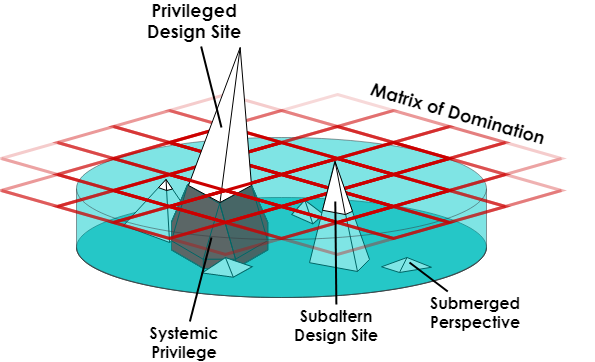
\includegraphics[height=3.5in]{figs/EST_Matrix of Dom_Submerged Perspectives.png}
  \caption[An illustration of the ``present'' point of the futures cone incorporating design justice concepts.]{A closer look at the conceptualization of a ``present" landscape which speculative futures will build upon, incorporating concepts from design justice to acknowledge histories of privilege and domination.}
  \label{fig:matrix-of-domination}
\end{figure}

In discussing our specific positionalities, we return to the combination of the speculative cone with intersectional design justice. Examining the present in more detail in Fig. \ref{fig:matrix-of-domination}, we can view what Costanza-Chock terms the \textit{matrix of domination} and how it systematically biases which futures are possible and plausible. This structure privileges certain design sites such as ``hackerspaces, makerspaces, and hackathons", while subjugating the majority of sociotechnical practice that takes place in marginalized and oppressed communities. These other sites under the matrix of domination, called \textit{subaltern design sites}, ``have always existed" in places such as weaving studios and auto shops, unacknowledged for their ingenuity. 
While the authors' individual identities privilege them differently in race and gender, we need to acknowledge our privilege as English-speaking, American practitioners working in privileged design sites: universities and tech start-ups. 
Our relationship-based methods thus limited our study socially and geographically, reflecting any existing privilege biases in our personal and professional networks. While some of our interviewees had previously worked in subaltern design sites for e-textiles, such as retail and production sewing, all their current positions were in similarly privileged sites. As a group primarily connected to other e-textiles practitioners in the USA and in Europe, our participant groups hardly included any colleagues from the Global South. 
To interrogate this limit, we add another element to the design justice landscape with a compatible concept from environmental justice, in the form of ``submerged perspectives" from G\'{o}mez-Barris' work in environmental justice with Indigenous communities in South America \cite{gomez-barris_extractive_2017}. This submerged position, also illustrated in Fig. \ref{fig:matrix-of-domination}, describes a geography of practices so obscured by the surface of colonialism and global capitalism that they find a certain form of autonomy from being invisible to the matrix of domination.  

The limitations in our conclusions represent opportunities for further inquiry, especially in supporting e-textiles practitioners from Indigenous and non-Western communities and their visions for sustainability. A design justice lens, focusing especially on a grassroots organizing ethos, lets us take stock of how we can use our findings and speculations in our own local communities of practice to find unique ways of doing sustainability. We actually see this lack of ``generalizability" as potential grounds for HCI and design inquiry into a multidimensional, globally diverse understanding of sustainable e-textiles development. 
% Returning to the issue of "scaling" as a tension in e-textiles collaborations, studies of cross-discipline conversations show that questions about how a novel idea "scales" can shut down participants and limit the generative capacity of brainstorming sessions \cite{niess_no_2020}. Yet, multiple definitions of ``scalability" exist simultaneously in manufacturing systems research \cite{putnik_scalability_2013}, suggesting that there may be multidimensional ways of understanding a global issue through globally diverse perspectives. 
We offer our method of \textit{speculative construction} as a prompt for \textit{retooling} for relationships and sustainable values as tactics for readers who wish to nurture their own communities of practice for sustainable development,  while staying humble in knowing that sustainability may be done differently elsewhere.

% We also saw that  We recognize that this omission severely limits the generalizability of our study's findings to a global e-textiles field, % CITE source explaining intention for using this term - postcolonial computing? HCI 4D
% WORDING: layers, histories, colonialism, post-colonial computing, speaks to discourses, systemic factors, problems with even choosing a geographic term to acknowledge these histories without perpetuating biases (e.g. "developing" countries)
% especially given the significant contributions to e-textiles in these regions (cite).
% Furthermore, we believe that we must prioritize improving % outreach to non-USA/European collaborators and sustainable e-textiles needs to consider global perspectives
% Global South is disproportionately affected by climate change due to histories of colonialism
% also have separate (by design) positions in manufacturing systems
% Vital in HCI4D and justice-based movements to consider postcolonial perspectives



% We couldn't spend a lot of time because ultimately, the timeline was decided by Flexsu's product development which in turn depended on their production. And sustainability is a hard topic to broach, so it was almost 99\% in speculations. 
% The beta test strongly suggested that we needed more than three weeks for a period of independent observation, perhaps treating such a study as more of a 6-week summer course. 
% cite: "time-deepening" in HCI work and "infrastructure" time, connect to discussions of "time" scales in sustainability scholarship
% However, with these now-established connections (which we are still maintaining), we now have more chances to go back and explore more.


% \todo[REWORK]{DISCUSSION, connecting it all back. describe how we intend for readers to take up ideas. and personally reflect on how creating "specuations' of systems we want is different than making design reccomendations for immediate action. perhpas its useful to reflect on the role of prototypes in this ecosystem - that some parts of our speculation relied on tools while others relied on other spaces. where can Hci come into play in this speculation}

% Even in e-textiles or computational design work that claims to address ``scalability", authors may be referring to different dimensions of scale. For example, 
% \cite{karimi_systems_2018} identifies the ``scalable" features of their prototype as cheap, nontoxic materials and compatibility with existing infrastructure, while 
% \cite{hennelly_makerspaces_2019} discussing ``scalability" as applied to makerspaces seems to emphasize the replicability dimension.

% Related to this last provocation is an array of other theoretical components of e-textiles technology, such as the meaning of ``infrastructure" and ``supply chain" in a sustainable manufacturing ecosystem, or the meanings of "lifecycle", "product", and "raw resource" if circularity and design for disassembly are assumed as alternative norms. Further theoretical inquiry into sustainable e-textiles -- be it deeper studies of language use in interdisciplinary e-textiles practices, systematic analyses of literature, or critical reviews that examine the (dis)organization of the domain corpus -- may not only yield insight into sustainable development tactics for the e-textiles field, but translatable insights for other technologies, as well.

\section{Crafting the Preferable Future(s)}

% Our work studied collaborative relationships in e-textiles and found all of this.
In summary, this work studied language use, prototyping, and manufacturing practices within the e-textiles/smart textiles field, an emergent interdisciplinary domain of technology. As e-textiles practitioners ourselves, we make the case for the specific stake which the e-textiles field holds in advancing intersectional sustainability, and are thus motivated to steer the field towards sustainable development in both academic and industry contexts. In observing how three aspects of e-textiles practice -- language, prototyping, and manufacturing -- shaped how practitioners formed and negotiated their collaborative relationships, we 
% (whose collaborative relationships between each other and with the study participants were reflexively part of the study) 
found themes of how these relationships were used to construct collective values in e-textiles development. In constructing the field as a shifting gestalt of relationships, we propose \keyterm{speculative construction} of sustainable e-textiles as a tactic for connecting e-textiles development to discourses in making sustainable, socio-ecological change.
% People form relationships for many purposes, usually to help themselves get to some goal. 
% Politics is all about organizing these relationships and negotiating goals to achieve a collective net gain. 
% "organizing" comes before "mobilizing". Establishing more connections also gives someone like me more soft power when pursuing a sustainability agenda.

To answer our original question of how sustainability manifests in ``material, implicit ways" in e-textiles, we expand on how interpersonal relationships drive e-textiles development. Literature in ethnographies of design, software development, STEM education, hardware prototyping, and many other areas of technological practice would corroborate the deeply emotional dimensions of work that is publicly constructed as objective and intellectual. However, our findings suggest that much work is needed to deconstruct manufacturing's template which is dominated by machines and minimizes human agency. 
% Our participants in the language, prototyping, and manufacturing segments led us to believe that, until someone deals with manufacturing first-hand in scaling new e-textiles technology, practitioners are generally not aware that manufacturing is more than solving a technical constraint. Rather, 
A significant portion of manufacturing is spent negotiating with other human stakeholders with expertise outside of the prototype's scope (e.g. supply chain, venture capital funding) and satisfying their requirements, assuming one can even get them in conversation. When talking to our manufacturing experts, the "supply chain" was not a matter of logistics and moving materials between places. Instead, the supply chain represented a series of gatekeepers who were frustratingly difficult to signal for attention. 

While this conceptualization of "scale" in e-textiles futures points to a need for educating interdisciplinary technologists on the business and social skills needed to advocate for their work, we argue a more radical position: that sustainable e-textiles practice needs to build relationships first, then design tools in response. The e-textiles field can seize upon existing relationship- and future-oriented practices to discuss sustainability critically, and beyond conversation (as talk is cheap yet necessary), actually develop more tools and tactics for sustainable e-textiles designs at inception. By forming coalitions across disciplinary boundaries, creating spaces to hold these boundaries between knowledge frameworks as subjects of agonistic examination, and provoking engagement with alternative infrastructures in software, hardware, and larger systems, we take this speculative construction as a site for \keyterm{retooling for sustainable e-textiles} workbenches of the future. Our scenes describe these tools not only as aspirational ideals, but also as actionable opportunities for designers.
% In closing, we offer one actionable conversational tactic for current e-textiles practitioners and those who are not yet in e-textiles: \textbf{Emphasizing that interpersonal, mutually beneficial relationships are as valuable as technical and creative skills for someone in e-textiles to be successful -- and centering that when creating projects and professional networks -- will scaffold sustainable mindsets in the field.} 
We contribute these tactics for e-textiles and allies in other HCI or ICT communities to orient themselves towards grassroots political organizing around sustainability, where forming and maintaining interpersonal relationships is part of making change, and more importantly, is where the most radically transformative work on sustainable futures is happening.

This collaboration with LOOMIA cemented ``retooling" as a keyword in my research practice, as it exposed me to design justice's definition that linked the technical process in engineering disciplines to the social and political implications of the infrastructural dynamic. From that definition, we were able to craft a theoretical contribution on designing future sustainable e-textiles, incorporating design justice with speculative design methods to critically reflect on whose speculations are prioritized. 
% As a note, this work is yet to be published after one submission/rejection cycle, and it is currently in a revise/resubmit phase after considering the reviewers' feedback. 
Taking this opportunity to reflect on a social research study that centered around conversations, I was reminded of coproduction from earlier work on AdaCAD that had continued to simmer in my theorizing of e-textiles design, which had not been a part of this work's framing and would perhaps strengthen the speculation. My realization-in-progress is how both coproduction and retooling are needed for a more insightful position on the societal impact of e-textiles. With just "coproduction" up to that point, I saw the collaborative and entangled aspects of e-textiles, but I had felt such a disconnect from how exactly to engage with that socio-political-technical ecosystem. Retooling offered a framework for literally obtaining the tools that I desired in order to surface the values that I wanted to see in e-textiles.
